%! TEX program =      xelatex
%! TEX bibliography = biber
%%%%%%%%%%%%%%%%%%%%%%%%%%%%%%%%%%%%%%%%%
% Journal Article
% LaTeX Template
% Version 1.4 (15/5/16)
%
% This template has been downloaded from:
% http://www.LaTeXTemplates.com
%
% Original author:
% Frits Wenneker (http://www.howtotex.com) with extensive modifications by
% Vel (vel@LaTeXTemplates.com)
%
% License:
% CC BY-NC-SA 3.0 (http://creativecommons.org/licenses/by-nc-sa/3.0/)
%
%%%%%%%%%%%%%%%%%%%%%%%%%%%%%%%%%%%%%%%%%

%----------------------------------------------------------------------------------------
%	PACKAGES AND OTHER DOCUMENT CONFIGURATIONS
%----------------------------------------------------------------------------------------

% \documentclass[twocolumn]{article}
\documentclass{article}
% allows for temporary adjustment of side margins
\usepackage{chngpage}
\usepackage{multirow}

\usepackage{blindtext} % Package to generate dummy text throughout this template

\usepackage[T1]{fontenc} % Use 8-bit encoding that has 256 glyphs
% \linespread{1.15} % Line spacing - Palatino needs more space between lines
\usepackage{microtype} % Slightly tweak font spacing for aesthetics

\usepackage[english]{babel} % Language hyphenation and typographical rules

% \usepackage[hmarginratio=1:1,top=32mm,columnsep=20pt]{geometry} % Document margins
% \usepackage[hang, small,labelfont=bf,up,textfont=it,up]{caption} % Custom captions under/above floats in tables or figures
\usepackage{booktabs} % Horizontal rules in tables

\usepackage{lettrine} % The lettrine is the first enlarged letter at the beginning of the text

\usepackage{enumitem} % Customized lists
\setlist[itemize]{noitemsep} % Make itemize lists more compact
\usepackage{graphicx}

\usepackage{abstract} % Allows abstract customization
\renewcommand{\abstractnamefont}{\normalfont\huge} % Set the "Abstract" text to bold
\renewcommand{\abstracttextfont}{\normalfont\small\itshape} % Set the abstract itself to small italic text

\usepackage{titlesec} % Allows customization of titles
% \renewcommand\thesubsection{\Roman{subsection}} % roman numerals for subsections
\titleformat{\section}[block]{\Large\scshape\centering}{\thesection}{1em}{} % Change the look of the section titles
% \titleformat{\subsection}[block]{\large}{\thesubsection}{1em}{} % Change the look of the section titles
% \titleformat{\subsubsection}[block]{\large}{\thesubsubsection}{1em}{} % Change the look of the section titles

\usepackage{fancyhdr} % Headers and footers
\fancyhead{} % Blank out the default header
\fancyfoot{} % Blank out the default footer
\fancyfoot[RO,LE]{\thepage} % Custom footer text

\usepackage{titling} % Customizing the title section

\usepackage{hyperref} % For hyperlinks in the PDF
\usepackage[style=authoryear,backend=biber,natbib=true,maxcitenames=2]{biblatex}
\addbibresource{bibliography.bib}
\usepackage{amssymb}
\usepackage{algorithm}
\usepackage{algpseudocode}

%----------------------------------------------------------------------------------------
%	TITLE SECTION
%----------------------------------------------------------------------------------------

\setlength{\droptitle}{-4\baselineskip} % Move the title up

\title{Face recognition through RGB-D images and matrices of SVMs} % Article title
\author{%
	\textsc{Federico Simonetta}\thanks{Ingegneria Informatica LM, matricola 1129912} \\[1ex] % Your name
	\normalsize \href{mailto:simonettaf@dei.unipd.it}{simonettaf@dei.unipd.it} % Your email address
	\and % Uncomment if 2 authors are required, duplicate these 4 lines if more
	\textsc{Alberto Cenzato}\thanks{Ingegneria Informatica LM, matricola 1134707} \\[1ex] % Your name
	\normalsize \href{mailto:alberto.cenzato@studenti.unipd.it}{alberto.cenzato@studenti.unipd.it} % Your email address
}
\date{\today} % Leave empty to omit a date
\renewcommand{\maketitlehookd}{%
	\begin{abstract}
		\noindent We tried to reimplement the algorithm described in \citet{Hayat2016}. We found that their results are reproducible with large datasets while with small datasets the SVM models have very low precision. We optimized the algorithm for two datasets of different size and tried several different preprocessing tweaks and decision algorithms. Lastly, we state that the biggest contributions to the good training of the SVMs are given by the size and the noiseness of the dataset and the accuracy of the preprocessing steps.
	\end{abstract}
}


\begin{document}

% Print the title
\Huge
\bfseries
\maketitle
\mdseries
\normalsize

\section{Introduction}\label{sec:intro}
\lettrine[nindent=0em,lines=2]{I}n \citet{Hayat2016} an algorithm for face recognition based on RGB-D image is given. RGB-D images are a state-of-the-art scene representation paradigm through which a 3D scene is described. Compared to classical RGB images, the RGB-D paradigm adds the Depth information that gives the chance to study images in a three-dimensional space. In their paper, Hayat et al.\ show that the Depth information can really raise precision of face recognition algorithms. \\
We tried to reproduce their results using a small dataset consisting of 338 images of 26 different individuals. Because of the very poor results, we tried to train the model with a new dataset of 20 different peoples in 24 sequences for a total of 15.678 RGB-D images \citep{Fanelli2013}. In \citet{Hayat2016}, authors used the second of these datasets, merged with other two datasets for a total of more than 35.000 images. \\
Our results let us think that this algorithm needs a very huge dataset for training.

\section{Algorithm description}\label{sec:algorithm_desc}
The algorithm proposed by \citet{Hayat2016} is roughly divided in three steps:
\begin{itemize}
	\item Detect the face and estimate its pose;
	\item Find a suitable feature space for the faces;
	\item Train the SVMs with the feature vectors obtained in the previous step.
\end{itemize}
These steps are briefly described in the next paragraphs. For a complete description see \citet{Hayat2016}.

\subsection{Normalization}\label{sec:normalization}
The input RGB-D images are preprocessed with a three steps pipeline. First step
in preprocessing is the background removal through a simple \textit{k}-means
clustering procedure on Depth images, the nearest cluster is the person. Then a
face detection and pose estimation algorithm is used \citep{Fanelli2013}.
Finally the pose information is used to precisely crop the face and RGB images
are converted to grayscale. \\
The basic idea is to look for the first non empty row from top in the segmented
Depth image, where \textit{non empty} means with at least $m$ non-zero pixels;
this is the top of the face ROI, lets call it $y_{top}$. $y_{top}$ is then
adjusted adding a factor proportional to the estimated head pose $$y_{top}' =
y_{top} + (\beta \phi +\gamma \psi)$$ where $\phi$ and $\psi$ are the
\textit{roll} and \textit{yaw} angles returned by the pose estimation of which
in \citet{Fanelli2011}, while $\beta$ and $\gamma$ are parameters set to $5/8$.
The ROI height is proportionally inverse to the distance of the head from the
camera $$y_{bottom} = y_{top} + 100/z$$ The cropping window position along the
\verb|X| axis is computed by looking for the first non empty column starting
from right and the first non empty column from left. \\

\subsection{Image subsets}
Once the cropped faces are available they are clustered based on their pose. For each person $c$ pose cluster centers are computed by \textit{k}-means; using these cluster centers, images of the person are assigned to one of the $c$ clusters based on the shortest euclidean distance between the cluster centers and the pose vector of each image.

\subsection{Image subsets representation}
Given a cluster of images from the same person a suitable representation for SVMs is computed:
\begin{itemize}
	\item each cropped image $j$ is divided in $4\times 4$ non-overlapping blocks;
	\item for each block, the LBP representation is computed;
	\item then the algorithm computes the difference $y(k, j)$ of each $k$-th LBP vector from its own mean;
	\item finally a $16\times16$ covariance matrix is computed by summing up all products between the standard deviations; in formula:
		$$C_{p, q} = \frac{1}{n} \sum_{i=1}^n y(p, i)y(q, i)$$
		where $i$ is the index of the image, $p$ and $q$ are respectively the row and the column index of the covariance matrix.
\end{itemize}

\subsection{SVMs}\label{sec:svm}
The covariance matrices are then used as a feature vector for the SVMs. $c \times N$ SVMs are trained (where $N$ is the number of people in the dataset) for the covariance matrices of the RGB images and just as many for the covariance matrices of the Depth images. All SVMs are binary classification SVMs trained in a one-vs-all fashion. \\
The SVMs use the Stein kernel function to map the covariance matrices (symmetric positive definite matrices) from Riemannian manifold to a high dimensional Hilbert space where they are linearly separable. The Stein kernel function is defined as
$$k(X,Y) = e^{-\sigma (\log{\det{\frac{X+Y}{2}}} - \frac{1}{2}\log{\det{XY}})}$$

\subsection{Fusion of results}
Once the SVMs are trained a query image set can be submitted to the algorithm. The image set must be of RGB and Depth image all of the same person. These images are preprocessed as in the training. The resulting $2c$ covariance matrices ($c$ for RGB and $c$ for Depth images) are classified by the $2c$ SVMs of each training person. The identity which receives the maximum number of ``votes'' is the predicted identity.
If more than one identity has the maximum number of votes, the one with the maximum distance from the hyper-plane is chose; if no SVM classifies the query covariance matrix with positive label, it is classified as \verb|unknown|.

\section{Algorithm implementation}\label{sec:algorithm_impl}
Our goal was to reproduce the results obtained by \citet{Hayat2016}. We implemented the algorithm in \verb|C++| and used the source code for random forest head pose estimation by \citet{Fanelli2013} as done by the authors. \verb|OpenCV| 3 was used both for image processing and SVM training and prediction. Two different implementations are the result of this work, one for each of the datasets we were provided with; they are more or less the same software with major differences only in the preprocessing steps which were tuned for the specific dataset they were made for.

\subsection{Datasets}\label{sec:datasets}
The first attempt was to adapt the algorithm by \citet{Hayat2016} on a small dataset containing 338 images of 26 different persons. This dataset contained:
\begin{itemize}
	\item frontal faces at 1 meter from the sensor;
	\item frontal faces at 2 meters from the sensor;
	\item non frontal faces at 1 meter from the sensor;
	\item frontal faces at 1 meter from the sensor with different expressions;
	\item variations in lighting;
	\item changing background scenes.
\end{itemize}
The very poor results obtained on this dataset forced us to implement all tweaks described in \ref{sec:background}, \ref{sec:cropping}, \ref{sec:training}. Anyway, our results did not agree with the results obtained in the paper. We can state with a reasonable certainty that the dataset was too small to train the model. \\
Therefore, we tested the algorithm on a new dataset by \citet{Fanelli2013}, containing almost half of the images used in \citet{Hayat2016}, with more than 15.000 images of 20 different persons. On this new dataset, Depth images were already segmented, therefore we removed the background segmentation step from the preprocessing pipeline. \\
From now on we will refer to the first dataset as \verb|dataset A| and the second as \verb|dataset B|.

\subsection{Background removal} \label{sec:background}
The first step in the preprocessing pipeline is to remove the background: a clean Depth image, with the person only, should be fed into the face cropping step (see \ref{sec:cropping}). Most of the effort in the implementation of the algorithm for \verb|dataset A| was put in this step. The task was not easy because of the non-uniform background in the images: the background was made of many objects and people at different Depths; it was not feasible to simply use a \textit{k}-means clustering as in \cite{Hayat2016} because the image did not have two obvious clusters. \\
In \verb|dataset B| this was already done on Depth images, so we have been able to skip this step. \\

\subsubsection{Face detection first}
A common error of \textit{k}-means clustering on \verb|dataset A| was to consider some objects and people slightly behind the individual of interest as part of his/her cluster. This produced a too loose cropping threshold resulting in an image with a partially removed background and making the pose estimation step \ref{sec:cropping} fail. We tried to overcome this introducing a face-detection step before clustering: only the face ROI was used for \textit{k}-means reducing the probability of clustering the wrong objects. If no face was detected, a fixed threshold segmentation was performed. \\
We used the Haar Cascades classifiers provided by OpenCV\footnote{For a presentation of the method see \href{https://docs.opencv.org/3.3.0/d7/d8b/tutorial_py_face_detection.html}{https://docs.opencv.org/3.3.0/d7/d8b/ \\
/tutorial\_py\_face\_detection.html} and \citet{ViolaJones}} to detect the face. \\
This method has three major disadvantages:
\begin{itemize}
	\item As known Haar Cascades classifiers are good at detecting frontal faces but their performance quickly decreases when processing non frontal or partially occluded faces. Moreover when many people are in the image it is difficult to say which one is the individual of interest;
	\item Of course it adds a computational cost;
	\item It is inefficient and redundant to perform a face detection in this phase since it will be done anyway in the pose estimation step \ref{sec:cropping}.
\end{itemize}

\subsubsection{Outlier removal}
After \textit{k}-means was applied all the background was removed, but many outliers to the right and the left of the person remained.
We traversed the image as a graph to find the connected components using \verb|connectedComponentsWithStats()| function from OpenCV. Only the component with the second maximum area was considered (the first should be the background): it was approximated with a rectangle and everything out of the bounding box was discarded.

\subsubsection{Dynamic segmentation with Depth histograms}
We also developed an algorithm able to dynamically segment Depth images with very good precision traded off against very long computation times. \\
To evaluate this new algorithm we gave a judgment of the segmentation quality on all the 338 images of the first dataset. Judgments were given with boolean values in reference to goodness of the segmentation of the main object represented in the pictures (in this case a person).	\\
Results gave 92.3\% of precision. Anyway, the longer computational time was not worth of the precision improvement (only 2\% more than the face-detection-first algorithm). However, this could be an improvement if very different images are used. \\
The algorithm was based on a histogram computation of Depth values and on the
assumption\footnote{We did not verified the assumption: studying in deep
this approach need first of all to check this assumption} that it was made of
``hills'', like a lots of Gaussians juxtaposed.
It looked for the most frequent value trying to estimate the range containing
the highest peak. If no face was detected in this range it was re-executed on
the second most high peak and so on. Estimation of the range was made
analyzing the logarithm of the second derivative, using fixed thresholds and
gradually enlarging the range. Maybe the most frequent value could be replaced
with the most large range, or the most wide area in a range.

\subsection{Face pose estimation and face cropping}	\label{sec:cropping}
In \citet{Hayat2016}, authors used the algorithm proposed in
\citet{Fanelli2011} to compute a face detection and pose estimation. We used
the same algorithm in the same way (see \ref{sec:normalization} for a brief
description of the algorithm and its parameters). However we chose to change
some of the parameters proposed in \citet{Hayat2016} for face cropping: $\beta
= \frac{15}{8}$, $y_{bottom} = y_{top} + \frac{120}{z}$. We used pose
estimation to correct ROI position along the \verb|X| axis too. When the person
is looking either to the left or to the right we crop the rear part of the head
with the following algorithm:
\begin{algorithm}
	\begin{algorithmic}[1]
		\If {$\theta$ > 0}
		\State $x_{base} = x_{base} - k \cdot |\theta|$
		\Else
		\State $x_{top} = x_{top} + k \cdot |\theta|$
		\EndIf
	\end{algorithmic}
\end{algorithm}
where $\theta$ is the head rotation around the vertical axis and $k = 1.5$ is a proportionality constant


\subsection{Image sets representation} \label{sec:covariances}
Next steps expected to cluster pose estimation converted from Euler angles to rotation matrix and to represent each cluster of each person with the covariance matrix described below. \\
We followed all of these steps, but we did not convert Euler angles given by the head pose estimation to rotation matrices; the pose estimation on \verb|dataset A| had some small errors which amplified when the rotation matrix was computed giving the wrong clustering. On \verb|dataset B| the pose estimation had an higher precision probably because it was the same dataset used by \citet{Fanelli2011}, but we used Euler angles clustering anyway.\\
After \textit{k-means} clustering we obtained $c=3$ clusters and ended up with $2\times c$ sets of images per person: $c$ sets of RGB images and $c$ sets of Depth images. The covariance matrices were computed as described in the paper.

\subsection{SVM training and prediction} \label{sec:training}
\begin{figure}
	\centering
	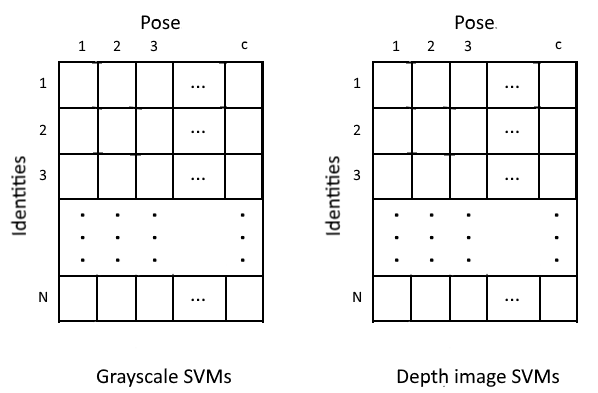
\includegraphics[width=\linewidth]{svms.png}
	\caption{
		\textbf{The SVMs matrices}: the algorithm trains $c$ SVMs for
		each identity on the RGB images (converted to grayscale) and
		$c$ SVMs for each identity on the Depth images. Each identity
		is associated in total to $2 \times c$ SVMs
	}
\end{figure}

To train the SVMs hyper-parameters\footnote{$C$, to regulate the soft margin, and $\sigma$, see \ref{sec:svm} for kernel function description.} we used the default parameter grid provided by OpenCV with logarithmic step. We evaluated each combination of parameters of each SVM with F-measure, so that only one true positive item existed. The final parameters chosen were the mean of the best performing parameters. \\
The paper was a bit ambiguous about the training strategy so we tried three different algorithms:
\begin{itemize}
	\item a simple training in which all covariance matrices but one had negative labels;
	\item a training in which all SVMs of the same correct identity had positive label;
	\item a training (only on the first dataset) in which the covariance matrix of the correct identity but of different poses were removed from the training set;
	\item \textit{leave-one-out}: only on the first dataset, without success; authors say that \textit{k-fold} cross validation gave low results.
\end{itemize}
The strategy to merge results from all the $2 \times N \times c$ SVMs was kept the same too, but we introduced a rule to achieve a better recognition of \verb|unknown| faces: if more than $t$ SVMs had the maximum number of votes, the face was forced to be \verb|unknown|. $t$ is a threshold that we set to $2c$, that is the maximum number of votes that each person should receive. This rule was quite effective: in our experiments it improved the final algorithm between the 10\% and the 40\% of \textit{rank-1}, while \textit{FP-unknown} was always 1. \\

\section{Experiments}
We made many experiments on \verb|dataset A| with no success. \\
From \verb|dataset B| we randomly extracted $40$ images from each person to be
used as testing set and 5 persons were completely removed from the training
set, to simulate the ``unknown'' behaviour. We never removed the persons that
have been recorded twice and for whom \verb|dataset B| contains two sets of
images. \\
We also used $\frac{1}{3}$ of the remaining training set as validation set to
evaluate SVMs performance and to find the best hyper-parameters. \\
As training strategy we used only the simple training described in
\ref{sec:training}. Note that a \textit{k}-fold cross validation may enhance
the results.

\section{Conclusions and results}
Our results differ a lot based on which identities were removed from the dataset. \\
This let us argue that our results still suffer for dataset size. Probably, a bigger dataset is needed to obtain good results. It is not the bigger number of image itself that would made the algorithm perform better, but it is a larger number of different identities: the average number of images per identity in \verb|dataset B| (about 700 images per identity) is much larger than in the final dataset used by the authors (about 300 images per identity). Actually, a greater number of identities means a greater number of covariance matrices and a greater number of items we can use to train the SVMs. This is coherent with Hayat's statement according to which the covariance set representation is very effective, in that it describes each person in a pose using a small number of images compared to other methods. \\

Also, we note that our results with RGB only or Depth images only are much lower than those claimed by the authors. We believe that in small datasets, Depth and RGB information merging is more useful because of the lack of items representative than in big datasets. \\

In the following tables we show our results achieved on multiple executions of the experiment with different combinations of `unknown'-`known' identities. Results are in terms of:
\begin{itemize}
	\item \textit{rank-1}: ratio between correct recognitions and the total number of queries, where `unknown' identities are considered correct if detected as `unknown';
	\item \textit{FP-unknown}: ratio between incorrect recognition of `unknown' persons and the total number of `unknown' persons.
\end{itemize}
Table \ref{tab:results-alpha} shows results obtained with the first version of the rule described in \ref{sec:training}, table \ref{tab:results-beta} shows results obtained using the second version (RGB images only).

\begin{table}[]
	\begin{adjustwidth}{-.75in}{-.75in}
		\centering
		\caption{Results with rule first version}
		\label{tab:results-alpha}
		\begin{tabular}{|l|l|c|l|c|l|c|}
			\hline
			\multirow{2}{*}{\bf Removed ids} & \multicolumn{2}{c|}{Using RGB-D images} &\multicolumn{2}{c|}{Using RGB images only} &\multicolumn{2}{c|}{Using D images only} \\ \cline{2-7}
							 & \bf Rank-1 & \bf FP-unknown            & \bf Rank-1 & \bf FP-unknown              & \bf Rank-1 & \bf FP-unknown  \\ \hline
			04, 06, 10, 11, 19               & 0.83	      & 0.4                       & 0.29       & 0.0                         & 0.33       & 0.4\\ \hline
			06, 10, 19, 20, 24               & 0.87	      & 0.0                       & 0.33       & 0.0                         & 0.50       & 0.0\\ \hline
			08, 09, 14, 17, 24               & 0.79	      & 0.4                       & 0.375      & 0.0                         & 0.33       & 0.2\\ \hline
			01, 16, 17, 19, 24               & 0.92	      & 0.2                       & 0.375      & 0.0                         & 0.42       & 0.2\\ \hline
			01, 09, 12, 16, 19               & 0.83	      & 0.6                       & 0.25       & 0.0                         & 0.375      & 0.4\\ \hline
			09, 10, 16, 19, 24               & 0.67	      & 0.8                       & 0.29       & 0.0                         & 0.125      & 0.8\\ \hline
			04, 09, 10, 11, 16               & 0.92	      & 0.2                       & 0.375      & 0.0                         & 0.33       & 0.2\\ \hline
			01, 08, 09, 10, 19               & 0.50	      & 0.8                       & 0.375      & 0.0                         & 0.125      & 0.6\\ \hline
			04, 10, 11, 13, 24               & 0.54	      & 1.0                       & 0.375      & 0.0                         & 0.20       & 0.0\\ \hline
			08, 14, 17, 23, 24               & 0.75	      & 0.6                       & 0.375      & 0.0                         & 0.29       & 0.6\\ \hline
			\bf mean                         & \bf 0.76   & \bf 0.5                   & \bf 0.3785 & \bf 0.0                     & \bf 0.33   & \bf 0.34\\ \hline
		\end{tabular}
	\end{adjustwidth}
\end{table}

\begin{table}[]
	\begin{adjustwidth}{-.75in}{-.75in}
		\centering
		\caption{Results with rule in second version}
		\label{tab:results-beta}
		\begin{tabular}{|l|l|c|l|c|l|c|}
			\hline
			\multirow{2}{*}{\bf Removed ids} & \multicolumn{2}{c|}{Using RGB-D images} &\multicolumn{2}{c|}{Using RGB images only} &\multicolumn{2}{c|}{Using D images only} \\ \cline{2-7}
							 & \bf Rank-1 & \bf FP-unknown            & \bf Rank-1 & \bf FP-unknown              & \bf Rank-1 & \bf FP-unknown  \\ \hline

			06, 09, 13, 17, 24               & 1.0        & 0.0                       & 0.33       & 0.0                         & 0.375      & 0.0\\ \hline

			06, 10, 11, 17, 20               & 0.92       & 0.0                       & 0.42       & 0.0                         & 0.54       & 0.0\\ \hline

			01, 09, 13, 14, 19               & 0.875      & 0.0                       & 0.42       & 0.0                         & 0.33       & 0.2\\ \hline

			04, 06, 11, 16, 17               & 0.79       & 0.0                       & 0.42       & 0.0                         & 0.42       & 0.2\\ \hline

			04, 11, 12, 17, 20               & 0.79       & 0.0                       & 0.29       & 0.0                         & 0.125      & 0.8\\ \hline

			04, 11, 12, 16, 23               & 0.71       & 0.0                       & 0.33       & 0.0                         & 0.08       & 1.0\\ \hline

			01, 06, 10, 17, 20               & 0.875      & 0.0                       & 0.375      & 0.0                         & 0.21       & 1.0\\ \hline

			10, 14, 16, 20, 24               & 0.92       & 0.0                       & 0.25       & 0.0                         & 0.375      & 0.0\\ \hline

			04, 06, 08, 14, 23               & 0.67       & 0.0                       & 0.33       & 0.0                         & 0.08       & 1.0\\ \hline

			04, 08, 11, 16, 20               & 0.92       & 0.0                       & 0.375      & 0.0                         & 0.08       & 1.0\\ \hline

			\bf mean                         & \bf 0.85   & \bf 0.0                   & \bf 0.354 & \bf 0.0                     & \bf 0.2615   & \bf 0.52\\ \hline
		\end{tabular}
	\end{adjustwidth}
\end{table}


\section{Technical considerations}

\subsection{Code and performance} \label{sec:code}
Hayat's algorithm is computationally intensive, therefore in our implementation we took care of using the entire processor's capacity and tried to avoid expensive operations. Both loading and preprocessing take advantage of a multi-threaded environment: images of a person are subdivided into $n$ sets, where $n$ is the number of concurrently executable threads on the machine, then each one of the $n$ threads is given a set to process. Cheap \verb|std::move()| operations were used whenever possible instead of copying data or passing error-prone pointers. \\
For \verb|dataset A| we used both OpenCV for RGB images and Point Cloud Library for loading Depth images. Depth images were then converted in OpenCV's \verb|cv::Mat| because Fanelli's face pose estimation algorithm needed Depth images in this format. For \verb|dataset B| PCL was not needed to load Depth images so we dropped it. \\

\subsection{Issues}
During the development we found many issues due to a beta stage of development  and the lack of complete documentation in OpenCV. Major issues were found in the use of machine learning module of OpenCV, namely in \textit{k}-means algorithm and in loading and saving custom kernel SVMs\footnote{Apparently there is no way of saving a custom kernel SMV without changing OpenCV's source code, loosing portability.}.

\section{Future developments}
The implementation could be improved both in terms of runtime performance and precision of the results. \\
Concerning the former, as said in \ref{sec:code}, some parts of the code are parallelized, while others are not, but could be. Both training and prediction could be executed concurrently on multiple SVMs. Furthermore the parallelization could took advantage of long processing pipelines avoiding to move data in and out the CPU's caches. Anyway this would result in a highly coupled code with no big processing gains. To obtain the highest grade of parallelization the code should be moved into a GPU-based approach, using OpenCV's \verb|cuda| module and implementing some custom CUDA kenerls when an operation is not available in \verb|cuda| module. \\
About the results instead we do not have a fair idea about why \textit{rank-1} results obtained by using RGB only images and Depth only images are so much poor with respect to the authors paper. This is the major issue we found in our results. \\
Another important point that should be clarified is to what extent the rule we introduced in prediction is useful. It should be tested on larger datasets. Moreover, we argued that the average number of images per person could be small, provided that the number of identities is big. This statement should be submitted to a more expansive investigation, by testing the algorithm with more identities and fewer images per identity. \\
Lastly, we kept track just of \textit{false positives} in the ``unknown'' prediction, but not of \textit{true positives}. We think that, according to the application, this could be a relevant measure of effectiveness.


\printbibliography

\end{document}
